\subsection{Merge-Sort:}

The program it's divided in four python modules to have a better control of the code:

\begin{itemize}
\item {\bfseries\itshape main.py:} Control the execution sequence, as well generate the list to sort and calls the {\bfseries\itshape Merge-Sort} algorithm.
\item {\bfseries\itshape mergesort.py:} Contains the {\bfseries\itshape Merge-Sort} algorithm.
\item {\bfseries\itshape merge.py:} Contains the {\bfseries\itshape Merge} algorithm.
\item {\bfseries\itshape graph.py:} Plot the {\bfseries\itshape size} against the {\bfseries\itshape time} that the algorithms takes to sort the list generated in {\bfseries\itshape main.py}. 
\end{itemize}

\subsubsection{Main.py}

In main.py the program will ask the user to enter a number {\bfseries\itshape 'n'}, this parameter will be the size of a 'list' of random numbers between {\bfseries\itshape [ -100, 100 ]}. The method that does this process it's {\bfseries\itshape menu ( )}: \hfill \break

\begin{lstlisting}
def menu ( ):
    ans = 0
    print ( "\n\n\tMerge-Sort Algorithm:\n" )
    ans = int ( input ( "\tAdd the size of the list: " ) )
    return list ( np.random.randint ( -100, 100, size = ans ) )
\end{lstlisting} \hfill

When the call to {\bfseries\itshape menu ( )} ends, the method will return the 'list' of size {\bfseries\itshape 'n'} -Let's call this list {\bfseries\itshape A}-, then the program will send it to {\bfseries\itshape mergesort ( ... )} to begin the sorting process. But the program will not send the complete 'list' at the first time, as we can see in the code showed bellow, in line 4 there is a {\itshape for} loop, and will iterate from {\bfseries\itshape 0 to 'n'} where {\bfseries\itshape 'n'} it's the size of {\bfseries\itshape A}, in each {\itshape iteration} the loop will "split" {\bfseries\itshape A} in a sublist {\bfseries\itshape B} of size {\bfseries\itshape i}, where {\bfseries\itshape i} will be the index of the loop. In other words {\bfseries\itshape B = A [ 0, ..., i ]} and {\bfseries\itshape B} will be the 'list' that {\bfseries\itshape mergesort} will receive as parameters. This process has a reason to be, as we can see in the line 5, {\bfseries\itshape mergesort} returns 2 values, {\bfseries\itshape m} and {\bfseries\itshape param}, the first one it's the 'list' sorted, and the second one is a {\itshape tuple}, where the first element it's the {\bfseries\itshape size} of the list {\bfseries\itshape B} and the second element it's the {\bfseries\itshape computation time} that the algorithm takes to sort that 'list' {\bfseries\itshape ( [ Size ( n ), Time ( t ) ] )}. In line 6, the program will append the {\itshape tuple} to a new 'list' named {\bfseries\itshape parameters}. \hfill \break

\begin{lstlisting}
def main ( ):
    parameters, n = [ ], menu ( )
    print ( "\n\tList to sort: ", n )
    for i in range ( len ( n ) + 1 ):
        m, param = mergesort ( n [ :i ] )
        parameters.append ( param )
    print ( "\n\tSorted list:  ", m, "\n" )
    print ( "\tMergeSort Parameters: ", parameters, "\n" )
    graph ( parameters )
\end{lstlisting} \hfill

So then, the loop finish when {\bfseries\itshape B = A}. As result, we will have the list {\bfseries\itshape A} sorted, and all the {\bfseries\itshape parameters} from {\bfseries\itshape $B_{i}$ to A}. This parameters will help to plot the {\bfseries\itshape computation time} against the {\bfseries\itshape size} of {\bfseries\itshape A}.

\begin{figure}[H]
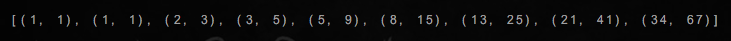
\includegraphics[scale=.65]{parameters.png}
\centering \linebreak \linebreak Figure 4.1.1.0: {\bfseries\itshape Parameters} list, where the first element it's the {\bfseries\itshape size} of {\bfseries\itshape $B_{i}$} and the second element it's the {\bfseries\itshape computation time} of {\bfseries\itshape mergesort}. The evaluated list it's of size {\bfseries\itshape n = 6} as we can see in the last {\itshape tuple}.
\end{figure}

\pagebreak

\subsubsection{Graph.py}

{\bfseries\itshape Graph ( ... )} plot {\bfseries\itshape Size ( n )} where {\bfseries\itshape 'n'} it's the length of {\bfseries\itshape A}, against {\bfseries\itshape Time ( t )} where {\bfseries\itshape t} it's the computational time that {\bfseries\itshape mergesort} takes to sort this list. As we can see, the parameters received it's the 'list' {\bfseries\itshape parameters}, as we said, this is a 'list' of tuples, and in every tuple we will have 2 elements a {\itshape size} and a {\itshape time}, well, this tuples will be the points to plot, so, the only thing rest to do is divide {\itshape parameters} into two lists, one for all the sizes, and another one for all the computational times, this process performed in the lines 8 and 10. \hfill \break

\begin{lstlisting}
def graph ( parameters ):
    # Window title.
    plt.figure ( "Merge-Sort Algorithm" )
    # Graph title.
    plt.title ( "Merge-Sort ( size, time ) = ( " + str ( parameters [ len ( parameters ) - 1 ] 
    	[ 0 ] ) + ", " + str ( parameters [ len ( parameters ) - 1 ] [ 1 ] ) + " )."  )
    # Parameter Time ( t ).
    t = list ( map ( lambda x: x [ 1 ], parameters ) )
    # Parameter Size ( n ).
    n = list ( map ( lambda x: x [ 0 ], parameters ) )
    # Proposed function g ( n ) = ( 3/2 ) ( n ) ( log ( n ) ).
    _t = list ( map ( lambda x: ( 3/2 ) * x, t ) )
    # Axes names.
    plt.xlabel ( "Size ( n )", color = ( 0.3, 0.4, 0.6 ), family = "cursive", 
    	size = "large" )
    plt.ylabel ( "Time ( t )", color = ( 0.3, 0.4, 0.6 ), family = "cursive", 
    	size = "large" )
    # Plot.
    plt.plot ( n, t, "#778899", linewidth = 3, label = "T ( n ) = ( n ) ( log ( n ) )" )
    plt.plot ( n, _t, "#800000", linestyle = "--", label = "g(n)=(3/2)(n)(log ( n ))")
    plt.legend ( loc = "upper left" )
    plt.show ( )
\end{lstlisting} \hfill

{\bfseries\itshape\color{armygreen}{Observation:}} {\itshape\color{armygreen}{We propose a function {\bfseries g( n ) = ( 3/2 ) ( n ) ( log ( n ) )}. In line 12, we take the elements of {\bfseries t} and multiply each one for ( 3/2 ), for later plot {\bfseries $t_{g( n )}$} against {\bfseries size ( n )}.}}

\subsubsection{Merge.py}

The function {\bfseries\itshape Merge ( ... )} it's very simply, takes two 'lists' and star to sort and combine those 'lists'. \hfill \break

{\bfseries\itshape\color{armygreen}{Observation:}} {\itshape\color{armygreen}{For now we will center on this code, in section 3.2 we will calculate the temporal complexity for this algorithm. And we will explain it more thoroughly}} \hfill \break

\begin{lstlisting}
def merge ( left, right ):
    m, i, j, time = [ ], 0, 0, 1
    # Convine and sort the lists 'left' and 'right'.
    while ( i < len ( left ) and j < len ( right ) ):
        time += 1
        if ( left [ i ] <= right [ j ] ):
            m.append ( left [ i ] )
            time += 1
            i += 1
            time += 1
        else:
            m.append ( right [ j ] )
            time += 1
            j += 1
            time += 1
    time += 1
    # The loop may break before all the rest of the elements in the lists
    # 'left' and 'right' are appended, hence, append the remaining elements.
    m.extend ( left [ i: ] )
    time += 2
    m.extend ( right [ j: ] )
    return m, time
\end{lstlisting}

\pagebreak

\subsubsection{Mergesort.py}

This it's the principal algorithm for this section, {\bfseries\itshape mergesort} will receive as parameter a 'list' -Let's name this 'list' {\bfseries\itshape A}-, of integer elements, and, if the length of {\bfseries\itshape A} it bigger than 1, then the algorithm will split {\bfseries\itshape A} in two halves, and will recursively call itself sending as parameter the first and the second half as we can see in lines 7 and 8, and will repeat this process until reaching the algorithm {\itshape bottom out}. \hfill \break

\begin{lstlisting}
def mergesort ( n ):
    # If the list has at most 1 element, return that list.
    if ( len ( n ) <= 1 ):
        return n
    # middle: Stores the integer length of the list splitted in 2.
    middle = int ( len ( n ) / 2 )
    left = mergesort ( n [ :middle ] )
    right = mergesort ( n [ middle: ] )
    # 'merge' convine and sort the left and right parts of the original list.
    return merge ( left, right )
\end{lstlisting} \hfill

As we can see in the code shown above, in line 10 we call {\bfseries\itshape merge ( ... )} so, the return statement will be a combined and sorted 'list'. To calculate the temporal complexity of this algorithm, we need to add a counter in each line {\bfseries\itshape ( time )}: \hfill \break

\begin{lstlisting}
def mergesort ( n ):
    time = 0
    # If the list has at most 1 element, return that list.
    if ( len ( n ) <= 1 ):
        return n, ( len ( n ), time )
    # middle: Stores the integer length of the list splitted in 2.
    middle = int ( len ( n ) / 2 )
    time += 1
    left, parameters = mergesort ( n [ :middle ] )
    time += 1 + parameters [ 1 ]
    right, parameters = mergesort ( n [ middle: ] )
    time += 1 + parameters [ 1 ]
    # 'merge' convine and sort the left and right parts of the original list.
    m, t = merge ( left, right )
    time += 1 + t
    return m, ( len ( n ), time )
\end{lstlisting} \hfill

Now, apart of return only the sorted and combined 'list', will return a tuple named {\bfseries\itshape parameters} ( The tuple {\itshape parameters} it's different than the 'list' with the same name that we talked about earlier
).  As we can see in line 16, {\bfseries parameters} inside has a counter named {\bfseries\itshape time}, this counter will not be the computational time of the algorithm unless we sum the other {\itshape times} of the recursively calls as we can see in lines 10 and 12. Thus, when the process it's finished, the algorithm will return {\bfseries\itshape A} sorted and a tuple with the {\bfseries\itshape length of A} and {\bfseries the computational time} that the algorithm takes to sort {\bfseries A}. \hfill \break

{\bfseries\itshape\color{armygreen}{Observation:}} {\itshape\color{armygreen}{The tuple {\bfseries parameters} returned in this algorithm in {\bfseries main.py} will become an element of the 'list' {\bfseries parameters}.}} \hfill \break

{\bfseries\itshape\color{armygreen}{Observation:}} {\itshape\color{armygreen}{As we can see in line 14, {\bfseries\itshape Merge} also return his computation time {\bfseries\itshape ( t )}, this value it's also summed to the counter of the temporal complexity of {\bfseries\itshape Merge-Sort}.}} 

\pagebreak